1. \begin{figure}[ht!]
\center{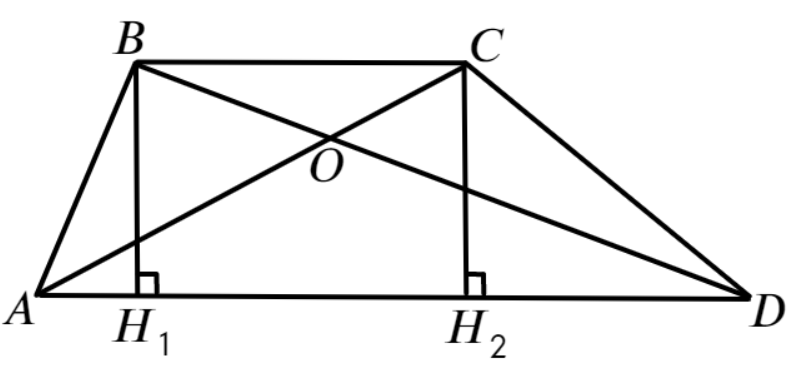
\includegraphics[scale=0.35]{g8-1.png}}
\end{figure}\\
Опустим высоты $BH_1$ и $CH_2.$ Тогда $BH_1H_2C$ является прямоугольником и $BH_1=CH_2.$ Поэтому $S_{\Delta ABD}=\cfrac{1}{2}BH_1\cdot AD=\cfrac{1}{2}CH_2\cdot AD=S_{\Delta ACD},$ значит $S_{\Delta AOB}=S_{\Delta ABD}-S_{\Delta AOD}=S_{\Delta ACD}-S_{\Delta AOD}=S_{\Delta COD},$ ч.т.д.\\
